\documentclass[12pt,addpoints,answers]{guia}
\grado{2$^\circ$ de Secundaria}
\cicloescolar{2022-2023}
\materia{Ciencias y Tecnología: Física}
\guia{3}
\unidad{3}
\title{Energía potencial}
%\unidad{3}
\title{El título de la guía}
\aprendizajes{\item Analiza la energía mecánica (cinética y potencial) y describe casos donde se conserva.
    }
\author{JC Melchor Pinto}
\begin{document}
\pagestyle{headandfoot}

\INFO
%\printanswers
\begin{opening}[Energía potencial gravitacional]{
        \begin{minipage}{0.45\textwidth}
            Si colocas un libro en la parte superior de un librero, utilizas una fuerza y lo
            desplazas cierta distancia; por tanto, requieres cierta energía para llevar a cabo el
            cambio en su posición, pero el libro, aun inmóvil, interactúa con la Tierra (lo que se
            manifiesta por su peso), puede caer y desplazarse una distancia. Debido a esta
            posibilidad se dice que el libro tiene energía potencial. Así, podemos definir la energía
            potencial gravitacional como la energía que tiene un cuerpo en virtud de su posición
            y que está relacionada con la fuerza de gravedad.
        \end{minipage}\hfill
        \begin{minipage}{0.55\textwidth}
            \begin{figure}[H]
                \centering
                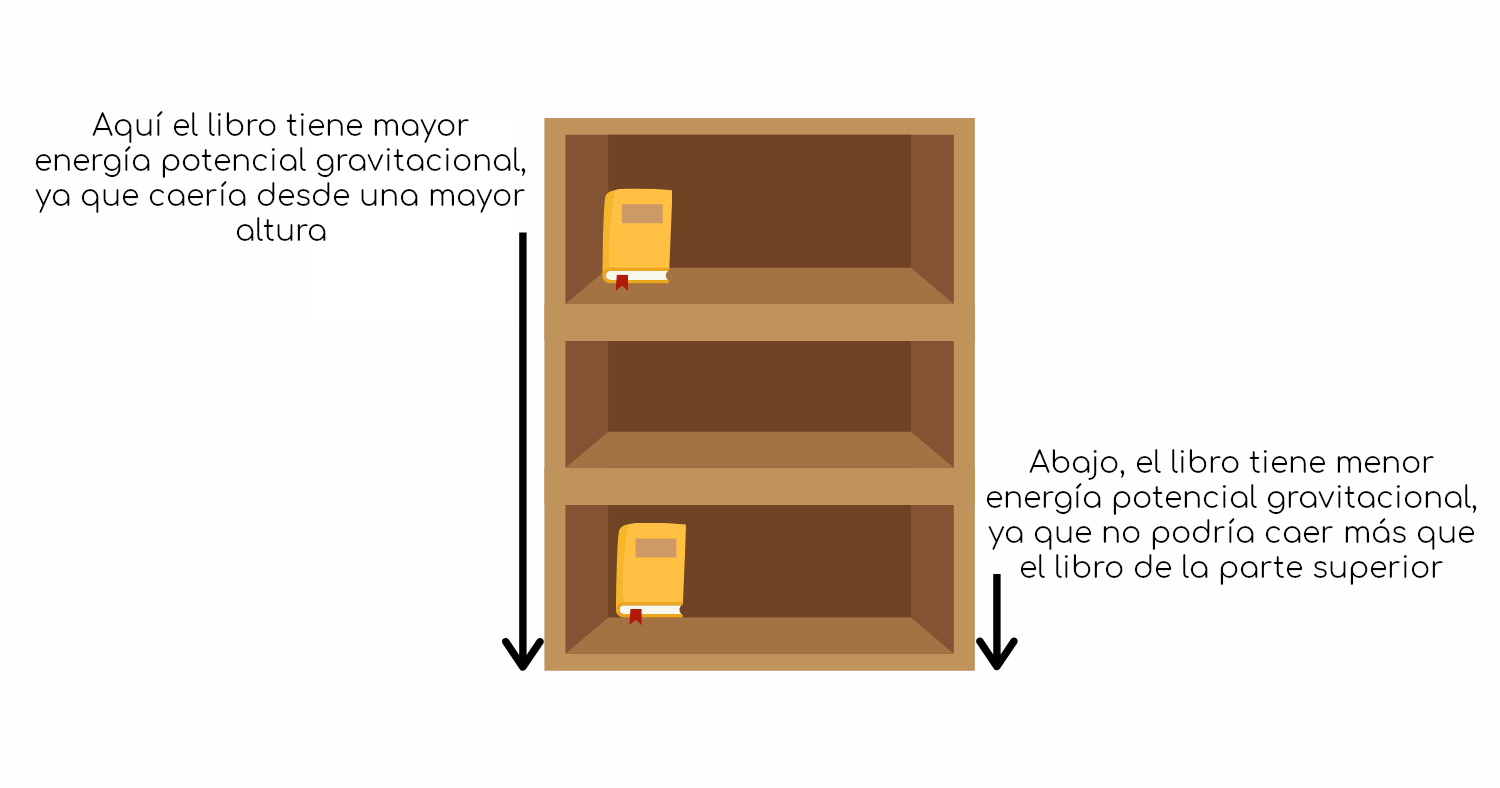
\includegraphics[width=\linewidth]{../images/Gravitational-potential-energy.png}
                %\captionof{figure}{Ejemplificación de la magnitud de la energía potencial gravitacional.}
                % \label{fig:gpe}
            \end{figure}%
        \end{minipage}

        La energía potencial depende de la altura del objeto con respecto a un marco de
        referencia, que puede ser la superficie terrestre, la mesa de trabajo, el pupitre,
        de modo que todo objeto que se encuentre en el origen de nuestro marco de referencia tendrá energía potencial gravitacional igual a cero. Mientras más alta sea la posición de un objeto en relación con el origen, mayores serán los cambios que pueda
        producir al interactuar con otros objetos y, por tanto, mayor será su energía potencial
        gravitacional.\\

        La energía potencial también depende de la masa de un cuerpo. Así, la
        ecuación para el cálculo de la energía potencial gravitacional (E$_p$) involucra
        a la masa de un cuerpo (m), la altura a la que se encuentra con respecto al
        marco de referencia (h) y la aceleración de la gravedad (g):
        \begin{equation}\label{potencial}
            E_p=mgh
        \end{equation}
        La unidad de la energía potencial, como la de la energía cinética, es el Joule (J).
    }
\end{opening}
\begin{questions}
    \newpage
    \include*{../questions/question011}
    \newpage
    \fullwidth{\begin{boxG}
            La ecuación (\ref{potencial}) requiere que las unidades de la masa sean expresadas en kilogramos (kg) y la altura en metros (m). Recuerda que el valor de la aceleración debido a la gravedad puede ser considerada como $g=9.8 \text{ m/s}^2$.
        \end{boxG}}
    \include*{../questions/question012}
    \include*{../questions/question013}
    \include*{../questions/question015}
    \newpage
    \fullwidth{\begin{boxG}
            De manera general, la ecuación (\ref{potencial}) puede ser utilizada para calcular cualquiera de las variables, incluyendo la masa del objeto y su altura. Para ello, deberas preparar la ecuación despejando la variable de tu interés.
            \begin{center}
                $E_p=mgh$ \qquad   $m=\dfrac{E_p}{gh}$ \qquad  $h=\dfrac{E_p}{mg}$
            \end{center}
        \end{boxG}}
    \include*{../questions/question014}
    \include*{../questions/question016}
    \newpage
    \include*{../questions/question020}
    \fullwidth{\begin{boxG}
            Cuando la altura de un objeto disminuye, desde un punto inicial a un punto final, la altura del objeto debe considerarse como negativa.
        \end{boxG}}
    \include*{../questions/question019}
    \include*{../questions/question017}

\end{questions}

%\vfill
%\puntuacion

\end{document}